\subsubsection{Decomposi\c c\~ao STL}\label{subsubsec:stl}




Através da decomposição, é possível analisar se a série apresenta tendência, sazonalidade e resíduos. Ao observar as Figuras \ref{fig:stl-aditiva} e \ref{fig:stl}, é evidente que os dados exibem ambos os padrões. Isso indica que a série é estacionária, como confirmado pelo seguinte teste.

\begin{figure}[!htb]
	\centering
	\caption{Decomposição STL aditiva dos dados coletados}
	\label{fig:stl-aditiva}
	\includegraphics[width=1\linewidth]{"Resultados/Figuras/STL aditiva"}
	
	
\end{figure}

\begin{figure}[!htb]
	\centering
	\caption{Decomposição STL multiplicativa dos dados coletados}
	\label{fig:stl}
	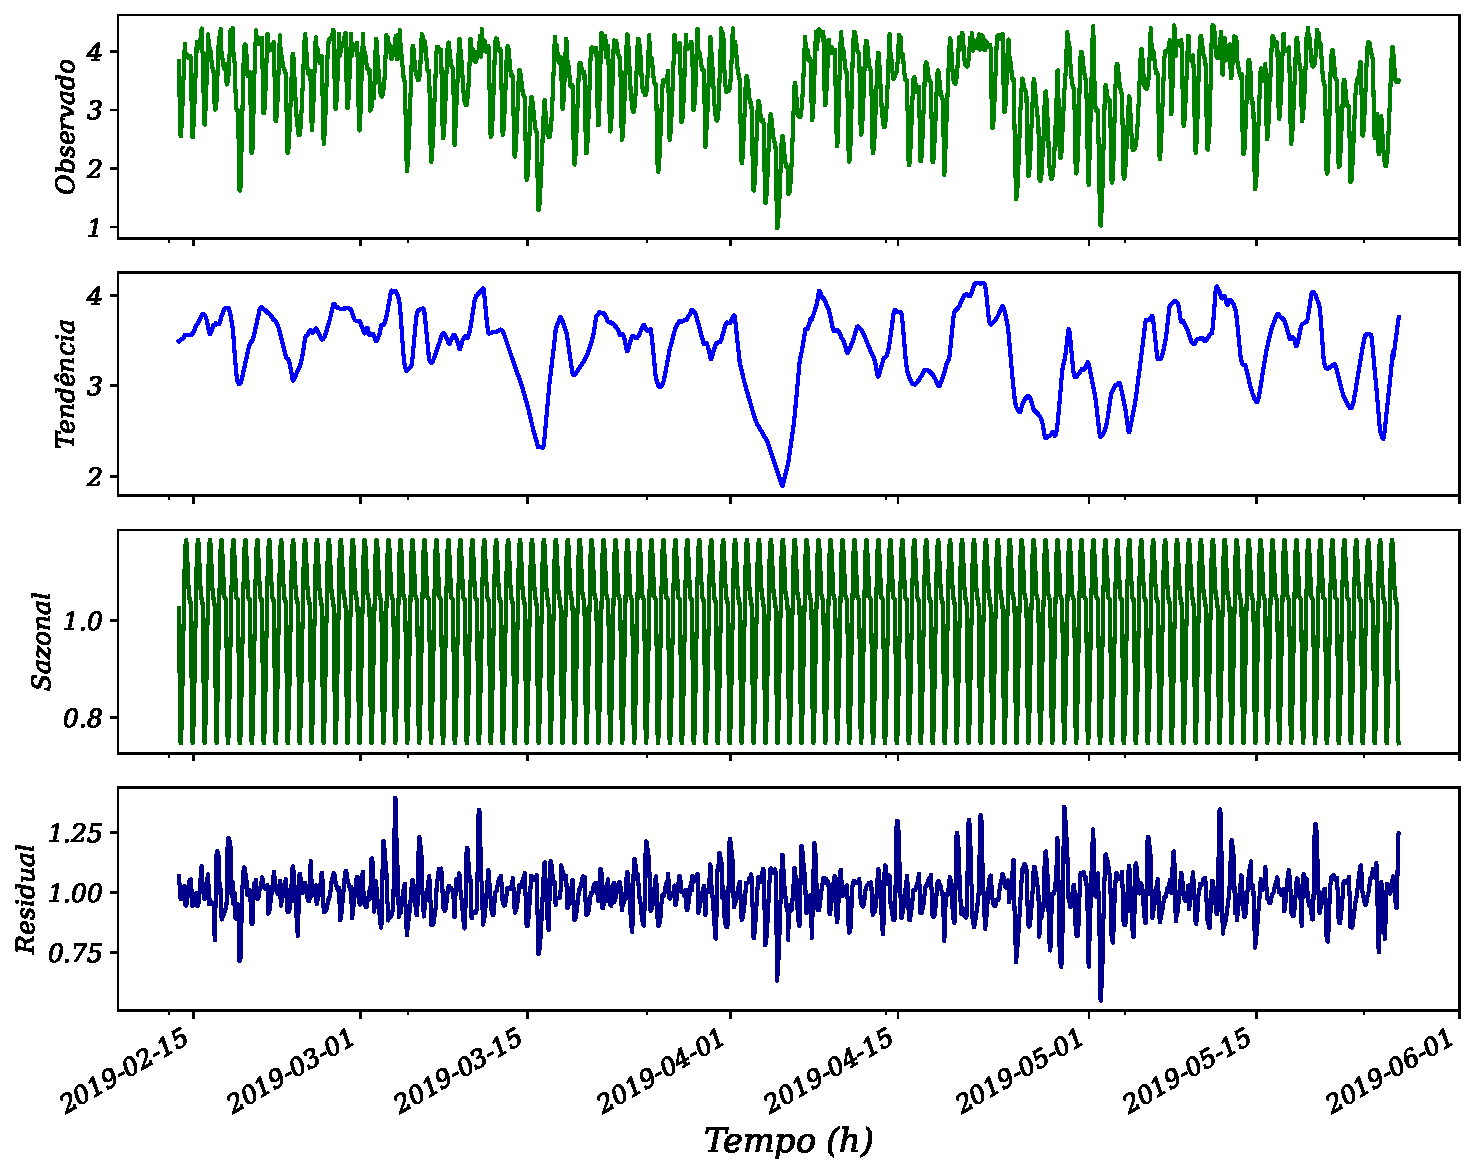
\includegraphics[width=1\linewidth]{Resultados/Figuras/STL}
		
	
	
\end{figure}



Teste de Dickey-Fuller (DF) Aumentado:
Estatística de teste ADF: $-4,25$;
Valor de p: $0,001$;
Atrasos utilizados: $21$;
Observações: $1074$;
Valor crítico ($1\%$): $-3,44$;
Valor crítico ($5\%$): $-2,86$;
Valor crítico ($10\%$): $-2,57$;
Com base na forte evidência contra a hipótese nula, podemos rejeitar a hipótese nula. A Figura \ref{fig:hist}, podemos notar um aumento na demanda durante essas horas durante o ano de 2019.
	
	
	\begin{figure}[!htb]
		\centering
		\caption{Violino no nível do reservatório}
		\label{fig:hist}
		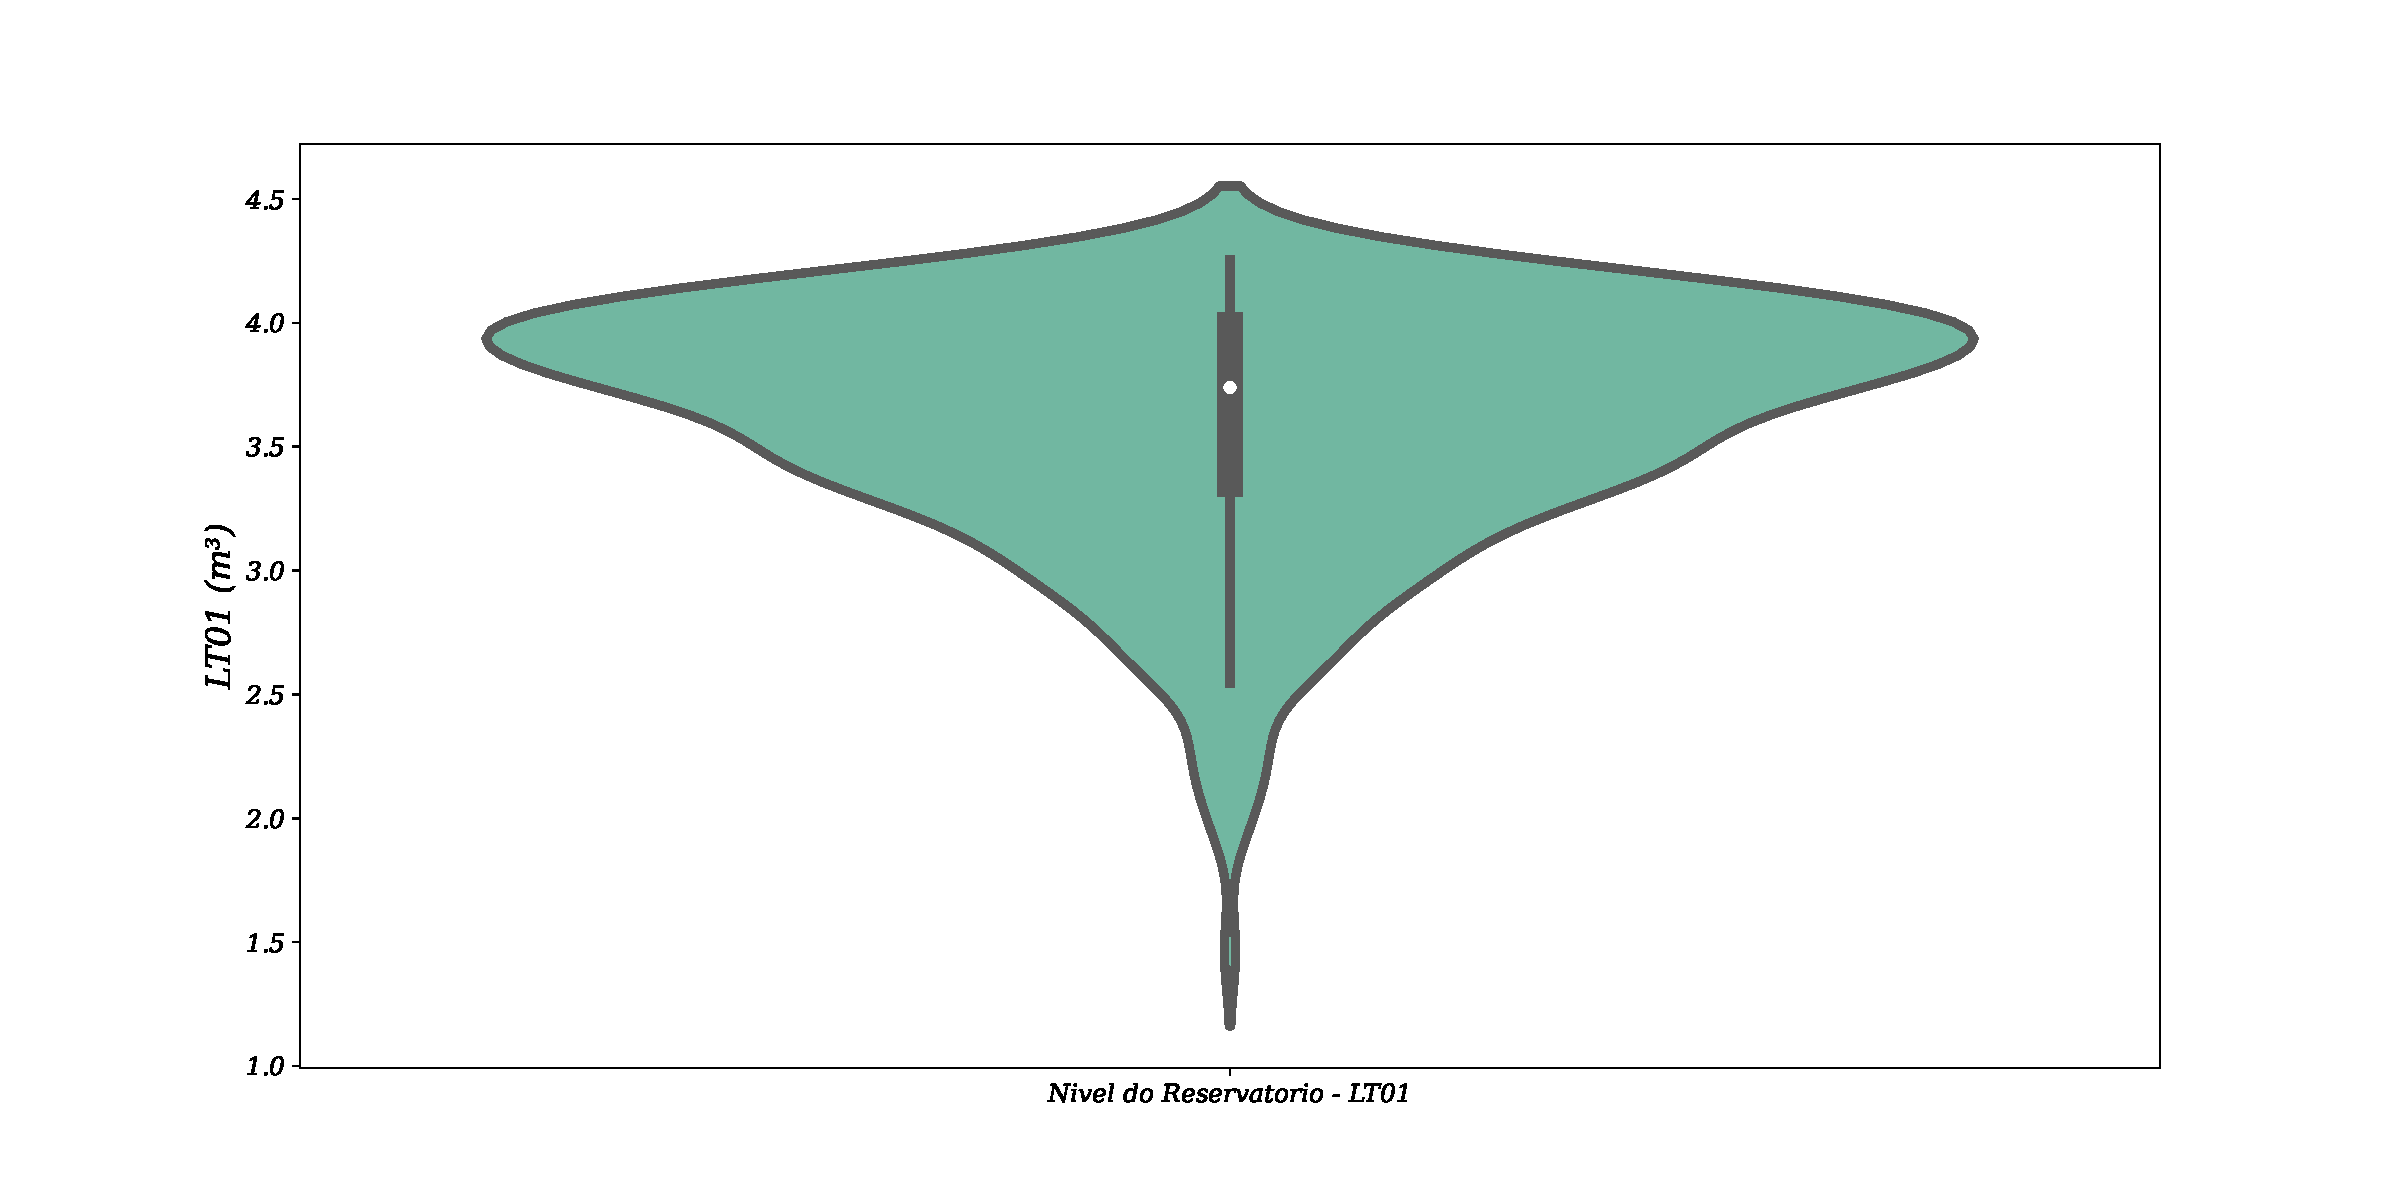
\includegraphics[width=0.9\linewidth]{Resultados/Figuras/viol}
		

	\end{figure}
	
Conforme mencionado na subseção \ref{subsubsec:motivacao}, as anomalias climáticas ocorridas em 2020, especialmente a falta de chuvas e devido ao COVID-19, tiveram um impacto significativo nos resultados. Isso contribuiu para as mudanças observadas na demanda de água ao longo desse período.



A Figura \ref{fig:ft03} ilustra como a vazão pode ser afetada pelo nível do tanque. É interessante observar que a vazão de recalque tem um impacto mais significativo no nível do tanque em comparação com as outras vazões. Isso ocorre porque a vazão de recalque está associada à injeção de água diretamente no tanque por meio da bomba localizada próxima à base do tanque. Por outro lado, as demais vazões apresentam alguns valores ausentes, o que limita sua influência na análise geral.	
	
	
	\begin{figure}[!htb]
		\centering
		\caption{Violino da vazão de recalque}
		\label{fig:ft03}
		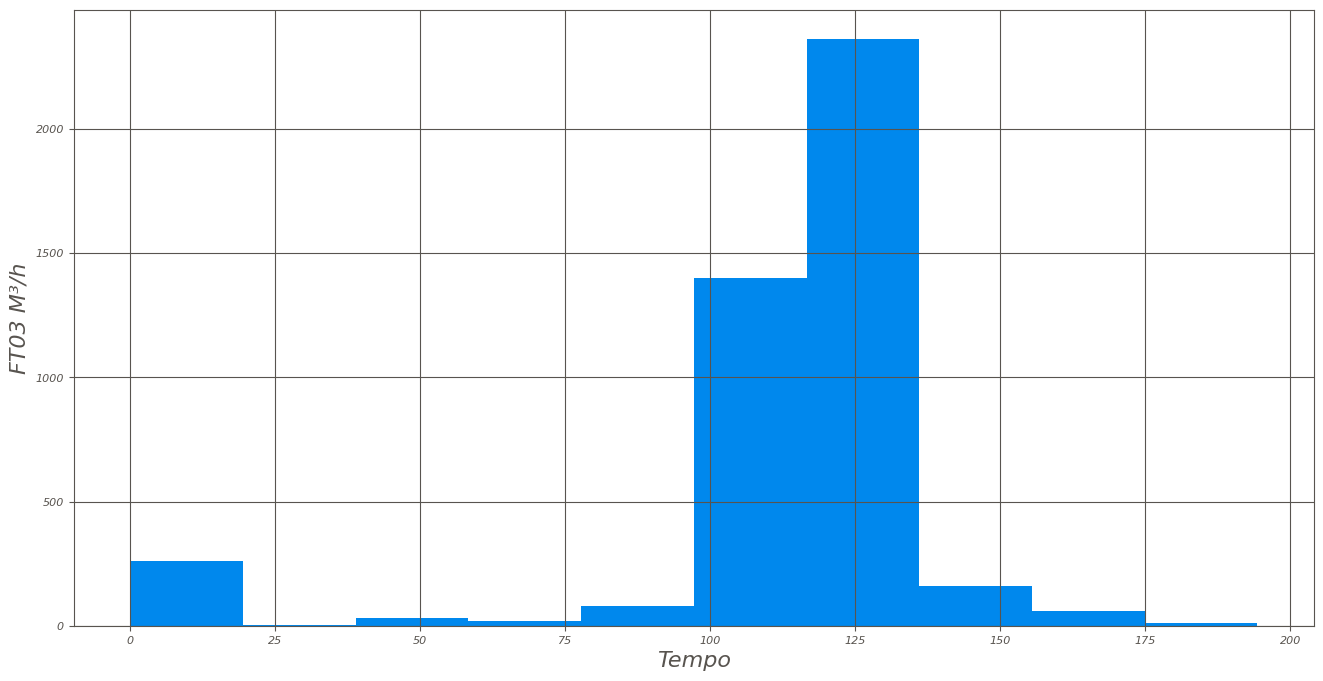
\includegraphics[width=0.9\linewidth]{Resultados/Figuras/ft03}
		

	\end{figure}


O ACF (do inglês \textit{Auto-Correlation Function}) é uma medida estatística utilizada para identificar a presença de correlação serial em uma série temporal. Ele calcula a autocorrelação entre os valores da série em diferentes defasagens, ou seja, a correlação entre os valores atuais e os valores passados da série. 

O ACF é útil para analisar a dependência temporal dos dados e identificar padrões de sazonalidade, tendência ou outros efeitos temporais. Por meio do ACF, é possível avaliar se a série exibe autocorrelação significativa em defasagens específicas, o que pode indicar a presença de não estacionariedade ou estrutura temporal que precisa ser considerada na análise ou modelagem da série temporal.

A estatística ADF (do inglês \textit{Augmented Dickey-Fuller}) de $-4,27$ indica a evidência de estacionariedade na série temporal. Quanto mais negativo for o valor da estatística ADF, maior é a evidência de estacionariedade nos dados.

O valor-p de $0,0005$, por sua vez, está associado ao teste ADF. O valor-p é uma medida estatística que representa a probabilidade de obter um resultado igual ou mais extremo do que o observado, sob a suposição de que a hipótese nula seja verdadeira. No caso do teste ADF, a hipótese nula é a presença de raiz unitária na série temporal, o que indica não estacionariedade. Assim, um valor-p baixo (geralmente abaixo de um nível de significância predefinido, como 0,05) sugere que a série temporal é estacionária, enquanto um valor-p alto sugere que a série temporal é não estacionária. Neste caso, o valor-p de $0,0005$ é bastante baixo, o que indica forte evidência contra a hipótese nula e sugere que a série temporal é estacionária.

Na Figura \ref{fig:acfa}, pode-se observar a diferença entre a autocorrelação (ACF) exibida na Figura \ref{fig:acfa} e a autocorrelação parcial (PACF) exibida na Figura \ref{fig:pacf}. A autocorrelação é uma medida da correlação entre os valores da série temporal em diferentes defasagens, levando em consideração tanto a correlação direta quanto a correlação indireta. Por outro lado, a autocorrelação parcial mede apenas a correlação direta entre os valores, desconsiderando a influência das defasagens intermediárias. Essas análises são úteis para identificar padrões e relações de dependência entre os valores da série temporal, fornecendo informações importantes para a modelagem e previsão desses dados.

\begin{figure}[!htb]
	\centering
	\caption{Autocorrelação}\label{fig:acfa}
	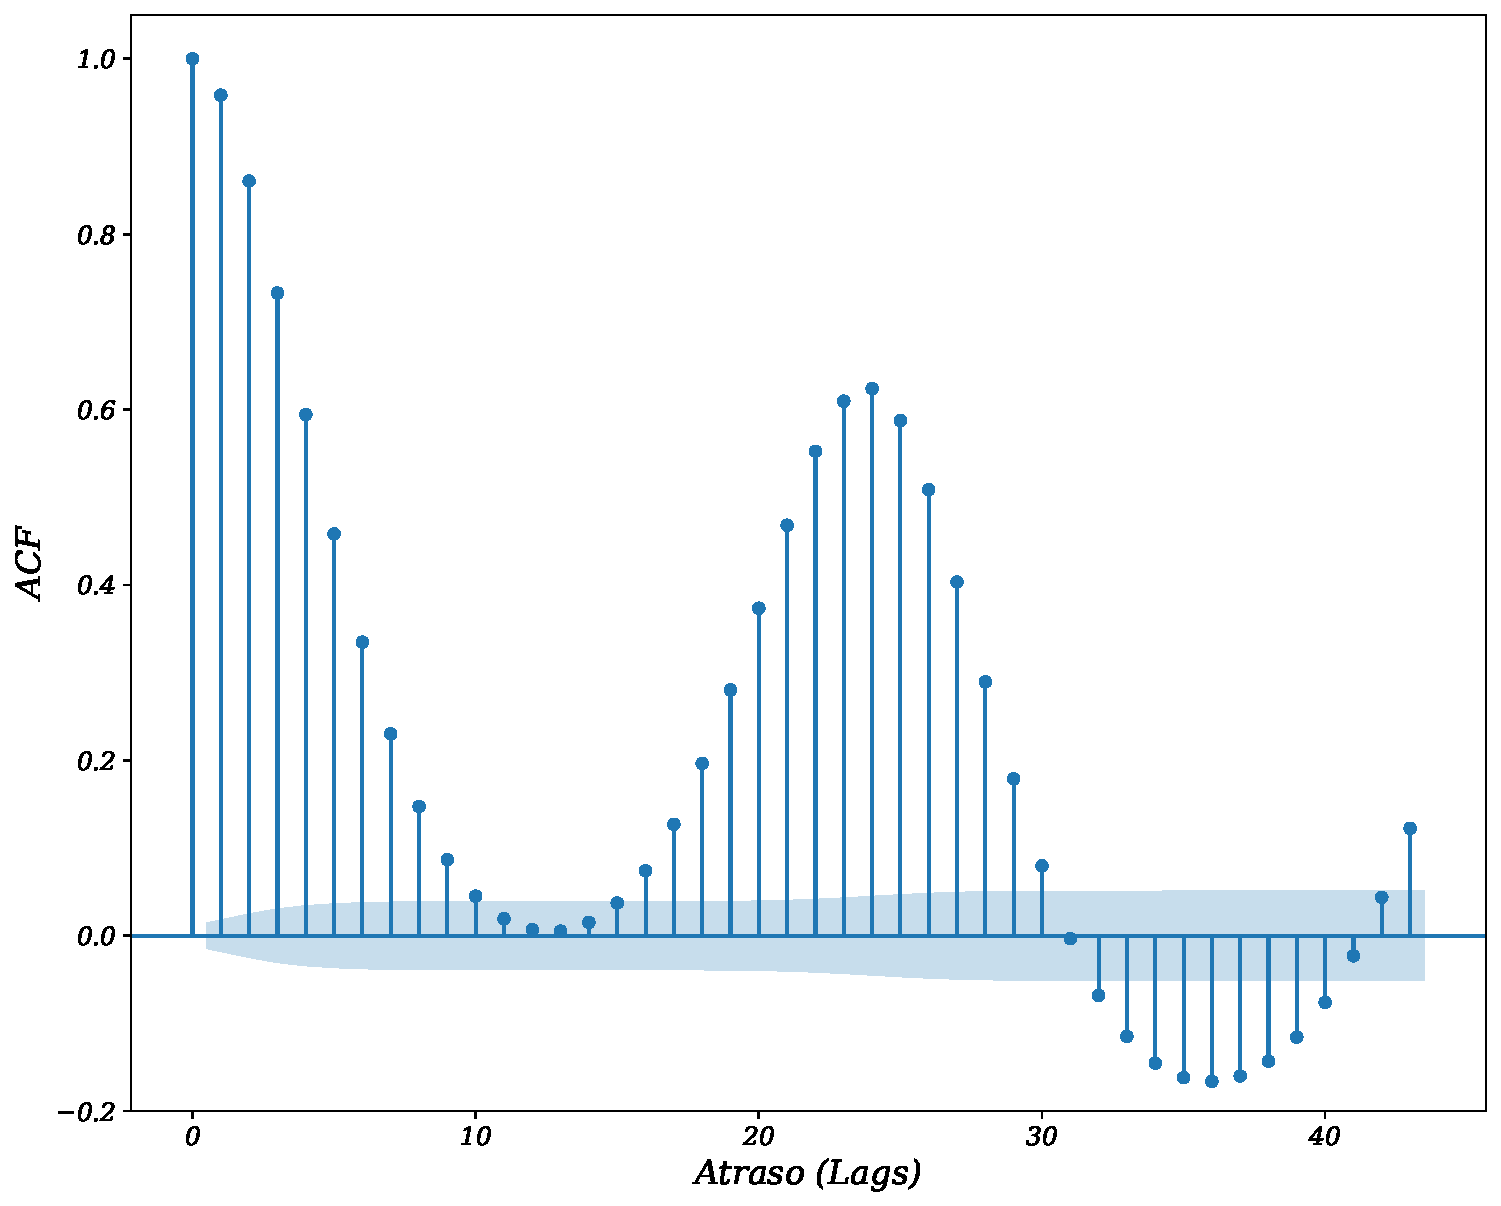
\includegraphics[width=0.9\linewidth]{Resultados/Figuras/acf} 
	

\end{figure}


\begin{figure}[!htb]
	\centering
	\caption{Autocorrelação parcial}\label{fig:pacf}
	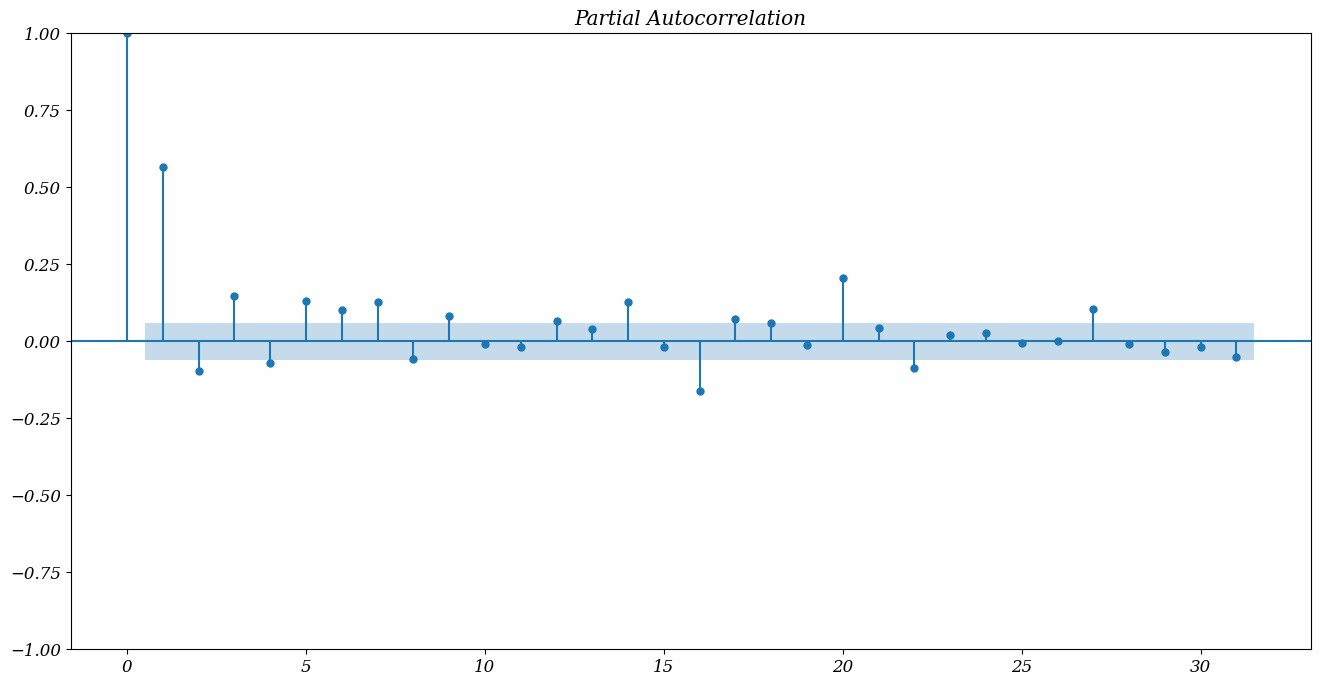
\includegraphics[width=0.9\linewidth]{Resultados/Figuras/pacf}
		
		

\end{figure}

O intervalo de confiança padrão de 95\% é representado pela marca azul na Figura. As observações que estão fora desse intervalo são consideradas estatisticamente correlacionadas, indicando a presença de padrões ou estrutura na série temporal.

A correlação visualizada na Figura \ref{fig:acfa} é fundamental para a interpretação do teste DF. Em uma série de ruído branco, os valores são completamente aleatórios e não apresentam correlação significativa. Portanto, quando há correlação presente na série, isso indica a existência de padrões ou dependências entre os valores, o que pode ser explorado para a modelagem e previsão da série temporal.


Na Figura \ref{fig:ruido-branco}, é possível observar uma série temporal que pode ser caracterizada como ruído branco. Uma série temporal é considerada ruído branco se suas variáveis forem independentes e distribuídas de forma idêntica, com média zero. Isso implica que todas as variáveis possuem a mesma variância ($\sigma^2$) e que cada valor não possui correlação com os demais valores da série.

\begin{figure}[H]
	\centering
	\caption{Ruído branco}
	\label{fig:ruido-branco}
	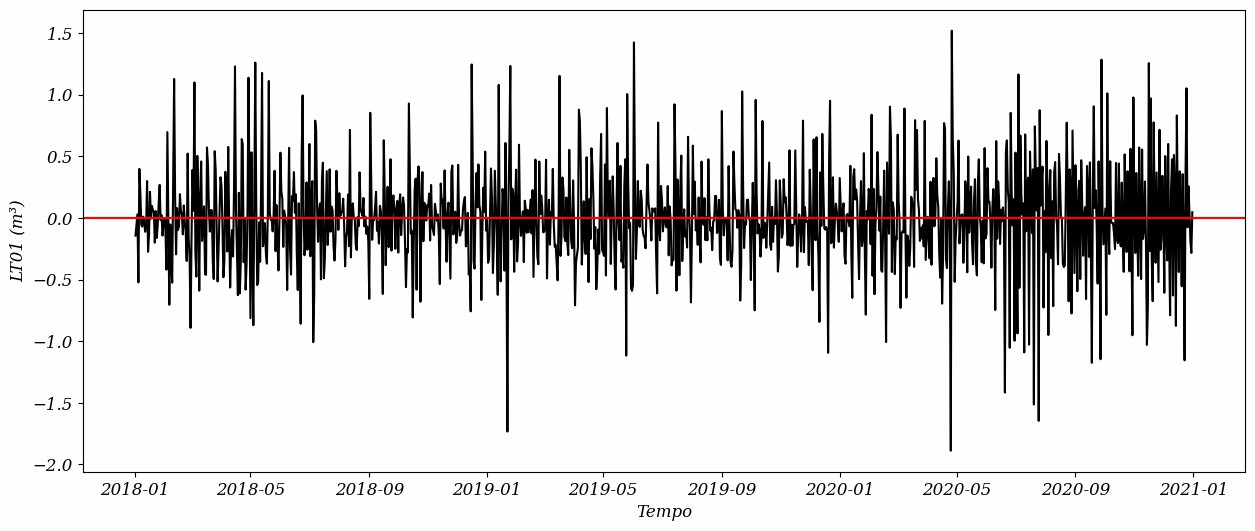
\includegraphics[width=0.9\linewidth]{Resultados/Figuras/ruido-branco}
	

\end{figure}
